\chapter{Psychological Science}

Science knows no country, because knowledge belongs to humanity, and is the torch which illuminates the world.
---Louis Pasteur
We live in a society exquisitely dependent on science and technology, in which hardly anyone knows anything about science and technology
---Carl Sagan



Many people believe that women tend to talk more than men---with some even suggesting that this difference has a biological basis. One widely cited estimate is that women speak 20,000 words per day on average and men speak only 7,000. This claim seems plausible, but is it true? A group of psychologists led by Matthias Mehl decided to find out. They checked to see if anyone had actually tried to count the daily number of words spoken by women and men. No one had. So these researchers conducted a study in which female and male college students (369 in all) wore audio recorders while they went about their lives. The result? The women spoke an average of 16,215 words per day and the men spoke an average of 15,669---an extremely small difference that could easily be explained by chance. In an article in the journal Science, these researchers summed up their findings as follows: "We therefore conclude, on the basis of available empirical evidence, that the widespread and highly publicized stereotype about female talkativeness is unfounded" \citep{mehl_are_2007}.

Science is a process for asking and answering questions about the world around. It is a powerful tool for changing our own minds about how we think the world works. For example, perhaps you too believed the stereotype that women are more talkative than men. If so, science has given you the opportunity to change your mind. The evidence collected so far shows that there are no virtually no differences in the number of words that women and men speak per day. If you choose to think like a scientist, then you ought to change your belief and strongly consider the possibility that the stereotype simply is not true. You might also read the published journal article from the research described above to critically evaluate how the research was conducted, and take a closer look at the patterns in the data. After all, if you want to update your beliefs on the basis of evidence, then you ought to make sure you can trust the evidence.

This course is an introduction to the process of using the scientific process to ask and answer questions relevant to psychologists. We will talk about how to critically evaluate scientific findings so that we can learn from the existing scientific literature. And, we will talk about how to collect data to ask questions, and how to analyze data to answer questions, so that we can contribute knowledge to the literature.

\section{Understanding Science}

\paragraph{Learning Objectives}
\begin{enumerate}
\item Define science.
\item Describe the three fundamental features of science.
\item Explain why psychology is a science.
\item Define pseudoscience and give some examples.
\end{enumerate}


Psychology is usually defined as the scientific study of human behavior and mental processes, and this example illustrates the features that make it scientific. In this chapter, we look closely at these features, introduce a model of scientific research in psychology, and address several basic questions that students often have about it. Who conducts scientific research in psychology? Why? Does scientific psychology tell us anything that common sense does not? Why should I bother to learn the scientific approach---especially if I want to be a clinical psychologist and not a researcher? These are extremely good questions, and answering them now will provide a solid foundation for learning the rest of the material in your course.

\subsection{What Is Science?}
Some people are surprised to learn that psychology is a science. They generally agree that astronomy, biology, and chemistry are sciences but wonder what psychology has in common with these other fields. Before answering this question, however, it is worth reflecting on what astronomy, biology, and chemistry have in common with each other. It is clearly not their subject matter. Astronomers study celestial bodies, biologists study living organisms, and chemists study matter and its properties. It is also not the equipment and techniques that they use. Few biologists would know what to do with a radio telescope, for example, and few chemists would know how to track a moose population in the wild. For these and other reasons, philosophers and scientists who have thought deeply about this question have concluded that what the sciences have in common is a general approach to understanding the natural world. Psychology is a science because it takes this same general approach to understanding one aspect of the natural world: human behavior.

\subsection{Features of Science}
The general scientific approach has three fundamental features \citep{stanovich_how_2013}. The  first is systematic empiricism. Empiricism refers to learning based on observation, and scientists learn about the natural world systematically, by carefully planning, making, recording, and analyzing observations of it. As we will see, logical reasoning and even creativity play important roles in science too, but scientists are unique in their insistence on checking their ideas about the way the world is against their systematic observations. Notice, for example, that Mehl and his colleagues did not trust other people's stereotypes or even their own informal observations. Instead, they systematically recorded, counted, and compared the number of words spoken by a large sample of women and men. Furthermore, when their systematic observations turned out to conflict with people's stereotypes, they trusted their systematic observations.

The second feature of the scientific approach---which follows in a straightforward way from the first---is that it is concerned with empirical questions. Empirical questions are questions that can be answered by observations. These are questions about the way the world actually is and, therefore, can be answered by systematically observing it. The question of whether women talk more than men is empirical in this way. Either women really do talk more than men or they do not, and this can be determined by systematically observing how much women and men actually talk. Having said this, there are many interesting and important questions that are not empirically testable and that science is not in a position to answer. Among these are questions about values---whether things are good or bad, just or unjust, or beautiful or ugly, and how the world ought to be. So, although the question of whether a stereotype is accurate or inaccurate is an empirically testable one that science can answer, the question---or, rather, the value judgment---of whether it is wrong for people to hold inaccurate stereotypes is not. Similarly, the question of whether criminal behavior has a genetic basis is an empirical question, but the question of what actions ought to be considered illegal is not. It is especially important for researchers in psychology to be mindful of this distinction.

The third feature of science is that it creates public knowledge. After asking their empirical questions, making their systematic observations, and drawing their conclusions, scientists publish their work. This usually means writing an article for publication in a professional journal, where they put their research question in the context of previous research, describe in detail the methods they used to answer their question, and clearly present their results and conclusions. Increasingly, scientists are opting to publish their work in open access journals so the articles are freely available to all -- scientists and nonscientists alike. This important choice allows publicly-funded research to create knowledge that is truly public.

Publication is an essential feature of science for two reasons. One is that science is a social process---a large-scale collaboration among many researchers distributed across both time and space. Our current scientific knowledge of most topics is based on many different studies conducted by many different researchers who have shared their work publicly over many years. The second is that publication allows science to be self-correcting. Individual scientists understand that, despite their best efforts, their methods can be flawed and their conclusions incorrect. Publication allows others in the scientific community to detect and correct these errors so that, over time, scientific knowledge increasingly reflects the way the world actually is.

A good example of the self-correcting nature of science is the "Many Labs Replication Project" -- a large and coordinated effort by prominent psychological scientists around the world to attempt to replicate findings from 13 classic and contemporary studies (Klein et al., 2013). One of the findings selected by these researchers for replication was the fascinating effect, first reported by Simone Schnall and her colleagues at the University of Plymouth, that washing one's hands leads people to view moral transgressions---ranging from keeping money inside a found wallet, to using a kitten for sexual arousal---as less wrong \citep{schnall_clean_2008}. If reliable, this effect might help explain why so many religious traditions associate physical cleanliness with moral purity. However, despite using the same materials and nearly identical procedures with a much larger sample, the "Many Labs" researchers were unable to replicate the original finding \citep{johnson_does_2014}, suggesting that the original finding may have stemmed from the relatively small sample size (which can lead to unreliable results) used in the original study. To be clear, at this stage we are still unable to definitively conclude that the handwashing effect does not exist; however, the effort that has gone into testing its reliability certainly demonstrates the collaborative and cautious nature of scientific progress.


\subsection{Science Versus Pseudoscience}

\paragraph{Skeptic's Dictionary}

The Skeptic's Dictionary is an excellent source for information on pseudoscience \url{http://www.skepdic.com}.
Among the pseudoscientific beliefs and practices you can learn about are the following:
\begin{itemize}
\item Cryptozoology. The study of "hidden" creatures like Bigfoot, the Loch Ness monster, and the chupacabra.
\item Pseudoscientific psychotherapies. Past-life regression, rebirthing therapy, and bioscream therapy, among others.
\item Homeopathy. The treatment of medical conditions using natural substances that have been diluted sometimes to the point of no longer being present.
\item Pyramidology. Odd theories about the origin and function of the Egyptian pyramids (e.g., that they were built by extraterrestrials) and the idea that pyramids in general have healing and other special powers.
\end{itemize}
Another excellent online resource is Neurobonkers \url{http://neurobonkers.com}, which regularly posts articles that investigate claims that pertain specifically to psychological science.


Pseudoscience refers to activities and beliefs that are claimed to be scientific by their proponents---and may appear to be scientific at first glance---but are not. Consider the theory of biorhythms (not to be confused with sleep cycles or other biological cycles that do have a scientific basis). The idea is that people's physical, intellectual, and emotional abilities run in cycles that begin when they are born and continue until they die. Allegedly, the physical cycle has a period of 23 days, the intellectual cycle a period of 33 days, and the emotional cycle a period of 28 days. So, for example, if you had the option of when to schedule an exam, you would want to schedule it for a time when your intellectual cycle will be at a high point. The theory of biorhythms has been around for more than 100 years, and you can find numerous popular books and websites about biorhythms, often containing impressive and scientific-sounding terms like sinusoidal wave and bioelectricity. The problem with biorhythms, however, is that there is simply no evidence for them, so there is no good reason to think they exist \citep{hines_comprehensive_1998}.

A set of beliefs or activities can be said to be pseudoscientific if (a) its adherents claim or imply that it is scientific, but (b) it lacks one or more of the three features of science. For instance, it might lack systematic empiricism. Either there is no relevant scientific research or, as in the case of biorhythms, there is relevant scientific research but it is ignored. It might also lack public knowledge. People who promote the beliefs or activities might claim to have conducted scientific research but never publish that research in a way that allows others to evaluate it.

A set of beliefs and activities might also be pseudoscientific because it does not address empirical questions. The philosopher Karl Popper was especially concerned with this idea \citep{popper_conjectures_2014}. He argued more specifically that any scientific claim must be expressed in such a way that there are observations that would---if they were made---count as evidence against the claim. In other words, scientific claims must be \emph{falsifiable}. The claim that women talk more than men is falsifiable because systematic observations could reveal either that they do talk more than men or that they do not. As an example of an unfalsifiable claim, consider that many people who believe in extrasensory perception (ESP) and other psychic powers claim that such powers can disappear when they are observed too closely. This makes it so that no possible observation would count as evidence against ESP. If a careful test of a self-proclaimed psychic showed that she predicted the future at better-than-chance levels, this would be consistent with the claim that she had psychic powers. But if she failed to predict the future at better-than-chance levels, this would also be consistent with the claim because her powers can supposedly disappear when they are observed too closely.

Why should we concern ourselves with pseudoscience? There are at least three reasons. One is that learning about pseudoscience helps bring the fundamental features of science---and their importance---into sharper focus. A second is that biorhythms, psychic powers, astrology, and many other pseudoscientific beliefs are widely held and are promoted on the Internet, on television, and in books and magazines. Far from being harmless, the promotion of these beliefs often results in great personal toll as, for example, believers in pseudoscience opt for "treatments" such as homeopathy for serious medical conditions instead of empirically-supported treatments. Learning what makes them pseudoscientific can help us to identify and evaluate such beliefs and practices when we encounter them. A third reason is that many pseudoscience's purport to explain some aspect of human behavior and mental processes, including biorhythms, astrology, graphology (handwriting analysis), and magnet therapy for pain control. It is important for students of psychology to distinguish their own field clearly from this "pseudo psychology."

\subsection{Key Takeaways}
\begin{fullwidth}
\begin{itemize}
\item Science is a general way of understanding the natural world. Its three fundamental features are systematic empiricism, empirical questions, and public knowledge.
\item Psychology is a science because it takes the scientific approach to understanding human behavior.
\item Pseudoscience refers to beliefs and activities that are claimed to be scientific but lack one or more
of the three features of science. It is important to distinguish the scientific approach to understanding human behavior from the many pseudoscientific approaches.
\end{itemize}
\end{fullwidth}

\subsection{Exercises}
\begin{fullwidth}
\begin{enumerate}
\item Practice: List three empirical questions about human behavior. List three nonempirical questions about human behavior.
\item Discussion: Consider the following psychological claim. "People's choice of spouse is strongly influenced by their perception of their own parents. Some choose a spouse who is similar in some way to one of their parents. Others choose a spouse who is different from one of their parents." Is this claim falsifiable? Why or why not?
\item Discussion: People sometimes suggest that psychology cannot be a science because either (a) human behavior cannot be predicted with perfect accuracy or (b) much of its subject matter (e.g., thoughts and feelings) cannot be observed directly. Do you agree or disagree with each of these ideas? Why?
\item Watch the following video by PHD Comics for an overview of open access publishing and why it matters. \url{https://www.youtube.com/watch?v=L5rVH1KGBCY}
\end{enumerate}
\end{fullwidth}

\newpage
\section{Scientific Research in Psychology}

\subsection{A Model of Scientific Research in Psychology}

\begin{figure}[0in]
      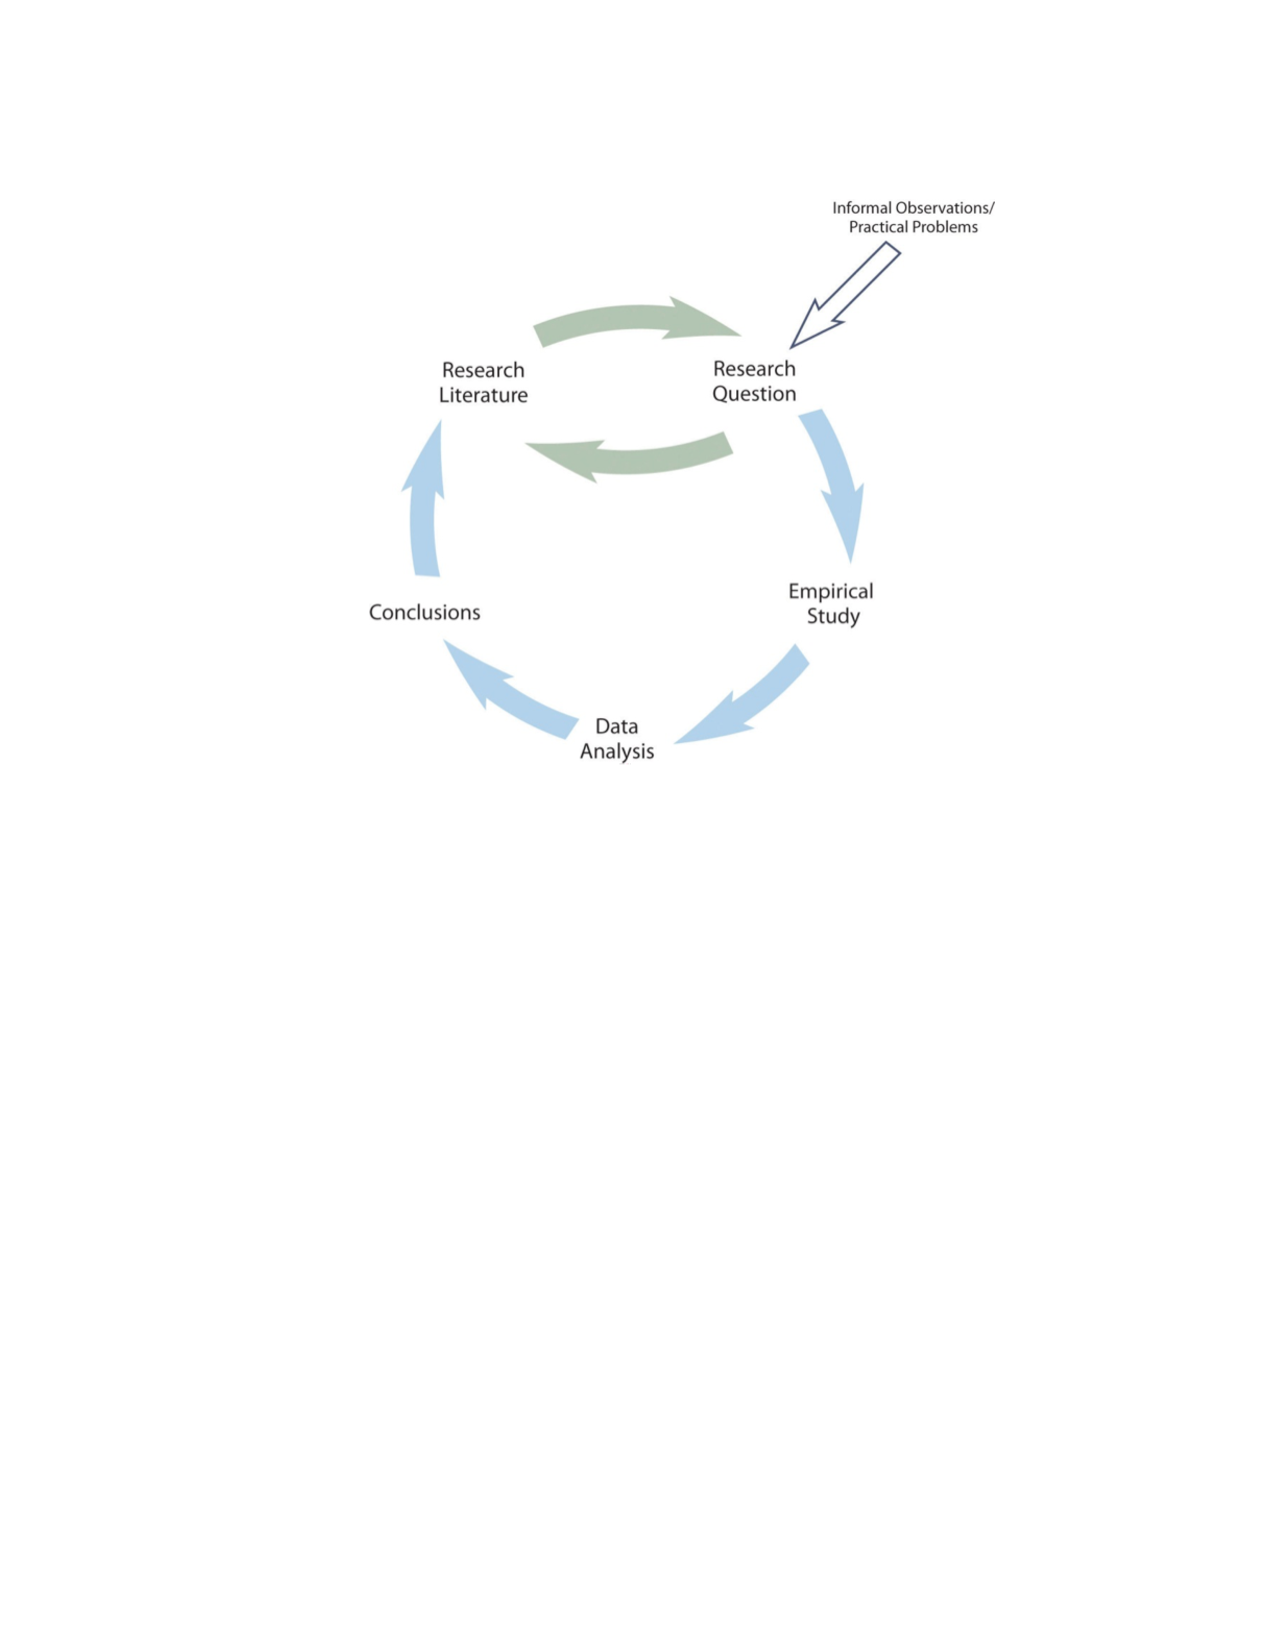
\includegraphics[width=\linewidth]{figures/C1Figure1.pdf}
      \caption{A simple model of scientific research in Psychology}
      \label{fig:Theresearchcycle}
\end{figure}

Figure \ref{fig:Theresearchcycle} presents a more specific model of scientific research in psychology. The researcher (who more often than not is really a small group of researchers) formulates a research question, conducts a study designed to answer the question, analyzes the resulting data, draws conclusions about the answer to the question, and publishes the results so that they become part of the research literature. Because the research literature is one of the primary sources of new research questions, this process can be thought of as a cycle. New research leads to new questions, which lead to new research, and so on. Figure \ref{fig:Theresearchcycle} also indicates that research questions can originate outside of this cycle either with informal observations or with practical problems that need to be solved. But even in these cases, the researcher would start by checking the research literature to see if the question had already been answered and to refine it based on what previous research had already found.

The research by Mehl and his colleagues is described nicely by this model. Their question---whether women are more talkative than men---was suggested to them both by people's stereotypes and by published claims about the relative talkativeness of women and men. When they checked the research literature, however, they found that this question had not been adequately addressed in scientific studies. They then conducted a careful empirical study, analyzed the results (finding very little difference between women and men), and published their work so that it became part of the research literature. The publication of their article is not the end of the story, however, because their work suggests many new questions (about the reliability of the result, about potential cultural differences, etc.) that will likely be taken up by them and by other researchers inspired by their work.

As another example, consider that as cell phones became more widespread during the 1990s, people began to wonder whether, and to what extent, cell phone use had a negative effect on driving. Many psychologists decided to tackle this question scientifically \citep{collet_phoning_2010}. It was clear from previously published research that engaging in a simple verbal task impairs performance on a perceptual or motor task carried out at the same time, but no one had studied the effect specifically of cell phone use on driving. Under carefully controlled conditions, these researchers compared people's driving performance while using a cell phone with their performance while not using a cell phone, both in the lab and on the road. They found that people's ability to detect road hazards, reaction time, and control of the vehicle were all impaired by cell phone use. Each new study was published and became part of the growing research literature on this topic.

\subsection{Who Conducts Scientific Research in Psychology?}

\paragraph{Scientific Psychology Blogs}

A fun and easy way to follow current scientific research in psychology is to read any of the many excellent blogs devoted to summarizing and commenting on new findings. Among them are the following:
\begin{itemize}
\item Brain Blogger \url{http://brainblogger.com/}
\item Mind Hacks \url{http://mindhacks.com/}
\item Research Digest \url{http://digest.bps.org.uk/}
\item Talk Psych \url{http://www.talkpsych.com/}
\item PsyBlog \url{http://www.spring.org.uk}
\item Social Psychology Eye \url{http://socialpsychologyeye.wordpress.com}
\item We're Only Human \url{http://www.psychologicalscience.org/onlyhuman}
\item You can also browse to \url{http://www.researchblogging.org}
\end{itemize}


Scientific research in psychology is generally conducted by people with doctoral degrees (usually the doctor of philosophy, PhD) and master's degrees in psychology and related fields, often supported by research assistants with bachelor's degrees or other relevant training. Some of them work for government agencies (e.g., the National Institute of Health), national associations (e.g., the American Psychological Association), nonprofit organizations (e.g., the Canadian Mental Health Association), or in the private sector (e.g., in product development). However, the majority of them are college and university faculty, who often collaborate with their graduate and undergraduate students. Although some researchers are trained and licensed as clinicians---especially those who conduct research in clinical psychology---the majority are not. Instead, they have expertise in one or more of the many other subfields of psychology: behavioral neuroscience, cognitive psychology, developmental psychology, personality psychology, social psychology, and so on. Doctoral-level researchers (post-doctoral fellows or research scientists) might be employed to conduct research full-time or, like many college and university faculty members, to conduct research in addition to teaching classes and serving their institution and community in other ways.

Of course, people also conduct research in psychology because they enjoy the intellectual and technical challenges involved and the satisfaction of contributing to scientific knowledge of human behavior. You might find that you enjoy the process too. If so, your college or university might offer opportunities to get involved in ongoing research as either a research assistant or a participant.

\paragraph{Many undergraduates at Brooklyn College volunteer in research labs in the Psychology Department, and can get course credit for their work by taking Independent Study or Research courses.}

Of course, you might find that you do not enjoy the process of conducting scientific research in psychology. But at least you will have a better understanding of where scientific knowledge in psychology comes from, an appreciation of its strengths and limitations, and an awareness of how it can be applied to solve practical problems in psychology and everyday life.

\subsection{The Broader Purposes of Scientific Research in Psychology}
People have always been curious about the natural world, including themselves and their behavior (in fact, this is probably why you are studying psychology in the first place). Science grew out of this natural curiosity and has become the best way to achieve detailed and accurate knowledge. Keep in mind that most of the phenomena and theories that fill psychology textbooks are the products of scientific research. In a typical introductory psychology textbook, for example, one can learn about specific cortical areas for language and perception, principles of classical and operant conditioning, biases in reasoning and judgment, and people's surprising tendency to obey those in positions of authority. And scientific research continues because what we know right now only scratches the surface of what we can know.

Scientific research is often classified as being either \emph{basic} or \emph{applied}. Basic research in psychology is conducted primarily for the sake of achieving a more detailed and accurate understanding of human behavior, without necessarily trying to address any particular practical problem. The research of Mehl and his colleagues falls into this category. Applied research is conducted primarily to address some practical problem. Research on the effects of cell phone use on driving, for example, was prompted by safety concerns and has led to the enactment of laws to limit this practice. Although the distinction between basic and applied research is convenient, it is not always clear-cut. For example, basic research on sex differences in talkativeness could eventually have an effect on how marriage therapy is practiced, and applied research on the effect of cell phone use on driving could produce new insights into basic processes of perception, attention, and action.

\subsection{Key Takeaways}
\begin{fullwidth}
\begin{itemize}
\item Research in psychology can be described by a simple cyclical model. A research question based on the research literature leads to an empirical study, the results of which are published and become part of the research literature.
\item Scientific research in psychology is conducted mainly by people with doctoral degrees in psychology and related fields, most of whom are college and university faculty members. They do so for professional and for personal reasons, as well as to contribute to scientific knowledge about human behavior.
\item Basic research is conducted to learn about human behavior for its own sake, and applied research is conducted to solve some practical problem. Both are valuable, and the distinction between the two is not always clear-cut.
\end{itemize}
\end{fullwidth}

\subsection{Exercises}
\begin{fullwidth}
\begin{enumerate}
\item Practice: Find a description of an empirical study in a professional journal or in one of the scientific psychology blogs. Then write a brief description of the research in terms of the cyclical model presented here. One or two sentences for each part of the cycle should suffice.
\item Practice: Based on your own experience or on things you have already learned about psychology, list three basic research questions and three applied research questions of interest to you.
\item Watch the following TED Ed video \url{https://youtu.be/ GUpd2HJHUt8}, in which David H. Schwartz provides an introduction to two types of empirical studies along with some methods that scientists use to increase the reliability of their results.
\end{enumerate}
\end{fullwidth}

\newpage
\section{Science and Common Sense}

\paragraph{Learning Objectives}
\begin{enumerate}
\item Explain the limitations of common sense when it comes to achieving a detailed and accurate understanding of human behavior.
\item Give several examples of common sense or folk psychology that are incorrect.
\item Define skepticism and its role in scientific psychology.
\end{enumerate}


\subsection{Can We Rely on Common Sense?}
Some people wonder whether the scientific approach to psychology is necessary. Can we not reach the same conclusions based on common sense or intuition? Certainly we all have intuitive beliefs about people's behavior, thoughts, and feelings---and these beliefs are collectively referred to as folk psychology. Although much of our folk psychology is probably reasonably accurate, it is clear that much of it is not. For example, most people believe that anger can be relieved by "letting it out"---perhaps by punching something or screaming loudly. Scientific research, however, has shown that this approach tends to leave people feeling more angry, not less \citep{bushman_does_2002}. Likewise, most people believe that no one would confess to a crime that he or she had not committed, unless perhaps that person was being physically tortured. But again, extensive empirical research has shown that false confessions are surprisingly common and occur for a variety of reasons \citep{kassin_psychology_2004}. There are many more examples where our own intuitions about ourselves and others are incorrect.

\subsection{How Could We Be So Wrong?}

\paragraph{Common Myths}

In 50 Great Myths of Popular Psychology, psychologist Scott Lilienfeld and colleagues \citep{lilienfeld_50_2011} discuss several widely held commonsense beliefs about human behavior that \emph{scientific research has shown to be incorrect}. Here is a short list:

\begin{itemize}
\item People use only 10\% of their brain power.
\item Most people experience a midlife crisis in their 40's or 50's."
\item Students learn best when teaching styles are matched to their learning styles."
\item Low self-esteem is a major cause of psychological problems."
\item Psychiatric admissions and crimes increase during full moons.
\end{itemize}


How can so many of our intuitive beliefs about human behavior be so wrong? Notice that this is an empirical question, and it just so happens that psychologists have conducted scientific research on it and identified many contributing factors \citep{gilovich_how_2008}. One is that forming detailed and accurate beliefs requires powers of observation, memory, and analysis to an extent that we do not naturally possess. It would be nearly impossible to count the number of words spoken by the women and men we happen to encounter, estimate the number of words they spoke per day, average these numbers for both groups, and compare them---all in our heads. This is why we tend to rely on mental shortcuts (what psychologists refer to as heuristics) in forming and maintaining our beliefs. For example, if a belief is widely shared---especially if it is endorsed by "experts"---and it makes intuitive sense, we tend to assume it is true. This is compounded by the fact that we then tend to focus on cases that confirm our intuitive beliefs and not on cases that dis-confirm them. This is called \emph{confirmation bias}. For example, once we begin to believe that women are more talkative than men, we tend to notice and remember talkative women and silent men but ignore or forget silent women and talkative men. We also hold incorrect beliefs in part because it would be nice if they were true. For example, many people believe that calorie-reducing diets are an effective long- term treatment for obesity, yet a thorough review of the scientific evidence has shown that they are not \citep{mann_medicares_2007}. People may continue to believe in the effectiveness of dieting in part because it gives them hope for losing weight if they are obese or makes them feel good about their own "self-control" if they are not.

\paragraph{Cognitive Biases}
Psychologists have identified numerous biases that influence how people think, reason, and make judgments about the world around them. Wikipedia maintains a long list of these biases that you can check out here: \url{https://en.wikipedia.org/wiki/List_of_cognitive_biases}


Scientists---especially psychologists---understand that they are just as susceptible as anyone else to intuitive but incorrect beliefs. This is why they cultivate an attitude of \emph{skepticism}. Being skeptical does not mean being cynical or distrustful, nor does it mean questioning every belief or claim one comes across (which would be impossible anyway). Instead, it means pausing to consider alternatives and to search for evidence---especially systematically collected empirical evidence---when there is enough at stake to justify doing so. For example, imagine that you read a magazine article claiming that giving children a weekly allowance is a good way to help them develop financial responsibility. This is an interesting and potentially important claim (especially if you have children of your own). Taking an attitude of skepticism, however, would mean pausing to ask whether it might be instead that receiving an allowance merely teaches children to spend money---perhaps even to be more materialistic. Taking an attitude of skepticism would also mean asking what evidence supports the original claim. Is the author a scientific researcher? Is any scientific evidence cited? If the issue was important enough, it might also mean turning to the research literature to see if anyone else had studied it. Then, you could evaluate the existing evidence yourself to determine whether the evidence supports the claim.

Because there is often not enough evidence to fully evaluate a belief or claim, scientists also cultivate a tolerance for uncertainty. They accept that there are many things that they simply do not know. For example, it turns out that there is no scientific evidence that receiving an allowance causes children to be more financially responsible, nor is there any scientific evidence that it causes them to be materialistic. Although this kind of uncertainty can be problematic from a practical perspective---for example, making it difficult to decide what to do when our children ask for an allowance---it is exciting from a scientific perspective. If we do not know the answer to an interesting and empirically testable question, science, and perhaps even you as a researcher, may be able to provide the answer.

\subsection{\allcaps{Key Takeaways}}
\begin{fullwidth}
\begin{itemize}
\item People's intuitions about human behavior, also known as folk psychology, often turn out to be wrong. This is one primary reason that psychology relies on science rather than common sense.
\item Researchers in psychology cultivate certain critical-thinking attitudes. One is skepticism. They search for evidence and consider alternatives before accepting a claim about human behavior as true. Another is tolerance for uncertainty. They withhold judgment about whether a claim is true or not when there is insufficient evidence to decide.
\end{itemize}
\end{fullwidth}

\subsection{\allcaps{Exercises}}
\begin{fullwidth}
\begin{enumerate}
\item Practice: For each of the following intuitive beliefs about human behavior, list three reasons that it might be true and three reasons that it might not be true:
\begin{itemize}
\item You cannot truly love another person unless you love yourself.
\item People who receive "crisis counseling" immediately after experiencing a traumatic event are better able to cope with that trauma in the long term.
\item Studying is most effective when it is always done in the same location.
\end{itemize}
\item Watch the following video, in which psychologist Scott Lilienfeld talks about confirmation bias, tunnel vision, and using evidence to evaluate the world around us \url{https://youtu.be/ Eut8jMfSA_k}
\end{enumerate}
\end{fullwidth}

\newpage
\section{Science and Clinical Practice}

\paragraph{Learning Objectives}

\begin{enumerate}
\item Define the clinical practice of psychology and distinguish it from the science of psychology.
\item Explain how science is relevant to clinical practice.
\item Define the concept of an empirically supported treatment and give some examples.
\end{enumerate}


Psychology is the scientific study of behavior and mental processes. But it is also the application of scientific research to "help people, organizations, and communities function better" (American Psychological Association, 2011). By far the most common and widely known application is the clinical practice of psychology---the diagnosis and treatment of psychological disorders and related problems. Let us use the term clinical practice broadly to refer to the activities of clinical and counseling psychologists, school psychologists, marriage and family therapists, licensed clinical social workers, and others who work with people individually or in small groups to identify and help address their psychological problems. It is important to consider the relationship between scientific research and clinical practice because many students are especially interested in clinical practice, perhaps even as a career.

\paragraph{Empirically Supported Treatments}

An empirically supported treatment is one that has been studied scientifically and shown to result in greater improvement than no treatment, a placebo, or some alternative treatment. These include many forms of psychotherapy, which can be as effective as standard drug therapies. Among the forms of psychotherapy with strong empirical support are the following:

\begin{itemize}
\item Cognitive behavioral therapy. For depression, panic disorder, bulimia nervosa, and post- traumatic stress disorder.
\item Exposure therapy. For post-traumatic stress disorder.
\item Behavioral therapy. For depression.
\item Behavioral couples therapy. For alcoholism and substance abuse.
\item Exposure therapy with response prevention. For obsessive-compulsive disorder.
\item Family therapy. For schizophrenia.
\end{itemize}

For a more complete list, see the following website, which is maintained by Division 12 of the American Psychological Association, the Society for Clinical Psychology  \url{http://www.div12.org/psychological- treatments}



The main point is that psychological disorders and other behavioral problems are part of the natural world. This means that questions about their nature, causes, and consequences are empirically testable and therefore subject to scientific study. As with other questions about human behavior, we cannot rely on our intuition or common sense for detailed and accurate answers. Consider, for example, that dozens of popular books and thousands of websites claim that adult children of alcoholics have a distinct personality profile, including low self-esteem, feelings of powerlessness, and difficulties with intimacy. Although this sounds plausible, scientific research has demonstrated that adult children of alcoholics are no more likely to have these problems than anybody else \citep{lilienfeld_50_2011}. Similarly, questions about whether a particular psychotherapy is effective are empirically testable questions that can be answered by scientific research. If a new psychotherapy is an effective treatment for depression, then systematic observation should reveal that depressed people who receive this psychotherapy improve more than a similar group of depressed people who do not receive this psychotherapy (or who receive some alternative treatment). Treatments that have been shown to work in this way are called \textbf{empirically supported treatments}.

Many in the clinical psychology community have argued that their field has not paid enough attention to scientific research---for example, by failing to use empirically supported treatments---and have suggested a variety of changes in the way clinicians are trained and treatments are evaluated and put into practice. Others believe that these claims are exaggerated and the suggested changes are unnecessary \citep{norcross_evidence-based_2006}. On both sides of the debate, however, there is agreement that a scientific approach to clinical psychology is essential if the goal is to diagnose and treat psychological problems based on detailed and accurate knowledge about those problems and the most effective treatments for them. So not only is it important for scientific research in clinical psychology to continue, but it is also important for clinicians who never conduct a scientific study themselves to be scientifically literate so that they can read and evaluate new research and make treatment decisions based on the best available evidence.

\subsection{\allcaps{Key Takeaways}}
\begin{fullwidth}
\begin{itemize}
\item The clinical practice of psychology—the diagnosis and treatment of psychological problems—is one important application of the scientific discipline of psychology.
\item Scientific research is relevant to clinical practice because it provides detailed and accurate knowledge about psychological problems and establishes whether treatments are effective.
\end{itemize}
\end{fullwidth}

\subsection{\allcaps{Exercises}}
\begin{fullwidth}
\begin{enumerate}
\item Discussion: Some clinicians argue that what they do is an “art form” based on intuition and personal experience and therefore cannot be evaluated scientifically. Write a paragraph about how satisfied you would be with such a clinician and why from each of three perspectives:
\begin{itemize}
\item a potential client of the clinician
\item a judge who must decide whether to allow the clinician to testify as an expert witness in a child abuse case
\item an insurance company representative who must decide whether to reimburse the clinician for his or her services
\end{itemize}
\item Practice: Create a short list of questions that a client could ask a clinician to determine whether he or she pays sufficient attention to scientific research.
\end{enumerate}
\end{fullwidth}

\section{Using Psychological Science to Inform Your Worldview}

Psychology is a very broad scientific discipline that asks and answers all sorts of questions about human and non-human animals. Psychological science encompasses many levels of analysis spanning the building blocks of biological systems, such as genes and cells, neurochemistry, neurons, and networks of neurons; perceptual and cognitive abilities of individuals such as learning, memory, attention, decision-making, language, thought, intelligence, and consciousness, to complex aspects of individuals such as development, personality, social behavior, and many others. A typical introductory psychology has the difficult job of presenting a bird's eye view of all of these major psychological domains of inquiry. Although psychologists ask many different kinds of questions, they all employ the scientific method as a tool to answer questions. So, this course is an introduction to the scientific research methods that are used in all areas of Psychology.

The primary focus of the course will be on experiments, which is the most powerful empirical tool researchers have to determine the underlying causes of the psychological phenomena that they measure. Psychological research methods are not limited to experiments, and non-experimental, or quasi-experimental approaches are often used with great success to ask and answer questions. Some of these research methods will be highlighted throughout the course.

\subsection{Why Should I Care About How Psychology Experiments work?}

Imagine for the moment a world without experiments that does not use the scientific method. This world would still have people claiming to have knowledge about how things work, and it would still have tools and technologies that are claimed to solve particular problems. However, without experiments to test whether the claims are true, all we are left with is the untested claims that may be true or false. We would be left in the dark. Inevitably, and not too different from our world today, there would be large segments of the population who believe false claims about how things work, and large segments of the population using therapies, tools, or other technologies that simply do not work (even if they believe they do).

The world we live in today discovered the scientific method and uses experiments to test claims about how things work. Indeed, with the enormous number of ways that we receive information through the media today, it is difficult to avoid hearing about all sorts of new scientific claims as well as totally unfounded claims that may not be based in science. For example, we have probably all heard that eating too much of something is good or bad for you, and increases or decreases your risk for a health problem. These claims can even flip around so that last year eating too much of X was bad, but this year eating too little of X is bad. What's more, many of these claims are supposedly scientific ones based on experiments. Should you believe these claims, and should you change your own behavior because of them?

 When we receive claims through the media we are getting second-hand information, and based on this information alone it is difficult to evaluate the claim and the evidence for the claim. One option is to find expert reporters that you trust, and then believe everything they say. The second option is to find the primary source, and then evaluate the evidence yourself to determine whether you should believe the claim. The ability to understand how experiments work gives you the tools you need to critically evaluate claims about how things work.

\subsection{Evaluating Claims}

It is an understatement to say that people believe all sorts of crazy things. Note, this is a claim that I just made. Should you believe it? What do you need to know to determine whether or not you should believe this claim or any other claim? Scientific thinking requires that claims are supported by evidence. Other forms of belief and thinking may not require evidence to support claims.

For the moment I'll put on my scientific thinking hat because there numerous ways that I can provide evidence for my claim the people believe all sorts of crazy things. I am a person, and I know that I have believed crazy things in the past. For example, when I was four I believed that all children grow to be taller than their parents because I visited a family who had many children of different ages, and the oldest ones were all taller than their parents. I believed this claim for many years until finding out at the age of 12 that all of the children in that family were adopted (nevertheless, I am taller than both my parents, but my brother is not, so much for my theory). The internet is full of people claiming to believe things that I think are completely crazy. For example, the flat earth society believes that the earth is flat and shaped like a frisbee. Believers in the great reptilian conspiracy maintain that many of our world leaders are lizard people. The abundance of conspiracy theories provides a deep well of evidence that people believe all sorts of crazy things. So, because I can back up my claim with evidence, I will continue believing that people believe all sorts of crazy things.

I could also take my science hat off, and then I can believe anything I want. Indeed, this remarkable imagination ability may be one reason why people believe so many crazy things without needing any evidence whatsoever to back up their beliefs. I can believe that I am a lizard monster who lives on a frisbee just because I want to. Indeed, the freedom to have your own opinion or belief about anything is a sacred cultural value in our western democracy. As citizens we respect each others right to their own opinions and beliefs. This is a way of respecting the right to have truthful and false and crazy beliefs, or respecting each others right to be completely wrong.

\subsection{Testable and Untestable Claims}
The scientific method for determining whether claims are true or false, or somewhere in the middle, has limitations because it can only be used to evaluate testable claims. A testable claim is one that makes a clear implication about a state of the world. For example, I claim that I have two hands. This is a testable claim because it clearly implies that if someone were to observe my arms, they would expect to find two hands at the end of them. If they did not find two hands, then they could dispatch with my claim because the evidence showed I had no hands, which would be in direct contradiction with the claim. An untestable claim is nonsensical, or does not make a clear implication about a state of the world. For example, consider the claim “aldfoha ofghnfsklhjas asdfilubhs”. This is just nonsense, and no one knows what it means, it does not make clear implications about a state of the world, so we will never know if it is true or false. Consider the claim “the members of the Zarkovian alien race from planet Zarko in a parallel universe all look like perfect glass spheres”. This claim is possibly sensible, because it could be tested if we could travel to that planet and find members of the Zarkovian race, but it is not practically testable because the needed evidence can not be gathered; so, we will never know if this made up claim is true or false, or almost true (perhaps they are cubes or ellipsoids).

Claims and evidence are two central parts of the scientific method. And, in psychological science neither of these parts come for free. Researchers construct both of them. One job is to create claims that can be tested. The other job is to make the evidence by creating situations necessary to conduct the tests. Joining the creation of claims with the creation of testable situations produces evidence that bears directly on the claim. The evidence can be consistent or inconsistent with the claim, allowing the claim to continue to be accepted or rejected.

Here is another claim: People don't always like to be wrong. I don't always like to be wrong, so at least there is one example. People have beliefs that are near and dear to their heart, so close perhaps, that a person might be devastated if they found out one of their precious ideas was wrong. For this reason, the evidence provided by scientific research may be viewed as a threat to a persons system of beliefs about the world. After all, when those beliefs involve testable claims, research can sometimes show those claims to be completely false. In which case, a rational person might be forced to delete parts of their beliefs that they would have preferred to hold on to. However, people aren't always rational and discovering evidence does not force anyone to do anything. For example, lots of research shows that people can persevere in maintaining false beliefs, even after they are told about the evidence showing their beliefs are false. So, people really do believe crazy things.

\subsection{Learning How Not To Be Crazy}
Learning about how experiments work is an opportunity to learn how not be crazy. Remember, experiments can only tell us about claims that can be tested, so we can not use this method to know whether our untestable beliefs are crazy. Fortunately, there are an endless number of testable claims that we can investigate that can add to the evergrowing library of human knowledge that science has produced so far, and be translated to applications that benefit ourselves, society, and the world around us.
